\documentclass[sigconf]{acmart}

% Language setting
\usepackage[english]{babel}

% Useful packages (acmart loads many common ones like amsmath, graphicx, hyperref, booktabs)
\usepackage{amssymb} % Loaded explicitly if specific symbols are needed beyond amsmath
\usepackage{tikz}
\usetikzlibrary{arrows.meta}
\usepackage[linesnumbered,ruled,vlined]{algorithm2e}
\usepackage{pgfplots} % For plots
\pgfplotsset{compat=1.18} % Recommended for current pgfplots versions

% algorithm2e setup
% \KwDownTo is a standard keyword in algorithm2e, no \SetKwDownTo needed.
\SetKwFor{For}{for}{do}{endfor}
\SetKwIF{If}{ElseIf}{Else}{if}{then}{else if}{else}{endif}
\SetKw{Nil}{NIL} % Define NIL keyword for consistency

%%
%% \BibTeX command to typeset BibTeX logo in the docs
\AtBeginDocument{%
  \providecommand\BibTeX{{%
    \normalfont B\kern-0.5em{\scshape i\kern-0.25em b}\kern-0.8em\TeX}}}

%% Rights management information. This information is sent to you
%% when you complete the rights form. These commands have SAMPLE values.
%% Please fill in the Values available to you from DIAGNOSTIC SCRIPT.
%% Example rights B:
\setcopyright{rightsretained}
% \setcopyright{acmcopyright}
\copyrightyear{2024} % Update as appropriate
\acmYear{2024} % Update as appropriate
% \acmDOI{XXXXXXX.XXXXXXX} % Update with your DOI

%% These commands are for a PROCEEDINGS abstract or paper.
% \acmConference[Conference acronym 'XX]{Make sure to enter the correct
%   conference title from your rights confirmation emai}{June 03--05,
%   2018}{Woodstock, NY}
% \acmPrice{15.00}
% \acmISBN{978-1-4503-XXXX-X/18/06}
% --- Replace with your actual conference info if applicable ---
\acmConference[SCSSL '24]{Workshop on Simple Cache-Sensitive Skip Lists}{Month DD, 2024}{City, Country}
\acmBooktitle{Proceedings of the Workshop on Simple Cache-Sensitive Skip Lists (SCSSL '24), Month DD, 2024, City, Country} % Fictional example
\acmPrice{0.00} % Or actual price
\acmDOI{10.1145/nnnnnnn.nnnnnnn} % Replace nnnnnnn
\acmISBN{978-x-xxxx-xxxx-x/YY/MM} % Replace with actual ISBN


\begin{document}

\title{A Simple Cache-Sensitive Skip List (SCSSL)}

\author{Yuchang Ke}
\email{aceking.ke@gmail.com}
\affiliation{%
  \institution{Your Institution Name Here} % TODO: Fill in
  \city{Your City} % TODO: Fill in
  \country{Your Country} % TODO: Fill in
}

\author{Bill Lv}
\email{ideaalloc@gmail.com}
\affiliation{%
  \institution{Your Institution Name Here} % TODO: Fill in
  \city{Your City} % TODO: Fill in
  \country{Your Country} % TODO: Fill in
}

\author{Weijie Zhang}
\email{zhangweijie@gmail.com}
\affiliation{%
  \institution{Your Institution Name Here} % TODO: Fill in
  \city{Your City} % TODO: Fill in
  \country{Your Country} % TODO: Fill in
}

%%
%% By default, the full list of authors will be used in the page
%% headers. Often, this list is too long, and will overlap
%% other information printed in the page headers. This command breaks
%% the author list for page headers. (Needed if more than 3 authors)
% \renewcommand{\shortauthors}{Ke, et al.}


\begin{abstract}
We present a cache-sensitive skip list (SCSSL) that is remarkably simple and easy to implement. It requires only minor modifications to the original skip list data structure to adapt it effectively to modern CPU architectures. This adaptation results in a performance improvement typically ranging from 1.2x to 1.6x, and on some systems, can reach 2x to 3x for insertion-heavy workloads.
Unlike other optimization techniques, SCSSL does not rely on specialized hardware instructions like SIMD or intricate multi-threaded programming paradigms. Instead, its design inherently benefits from improved data locality due to the use of arrays at the data level, a feature that modern compilers can further leverage. This makes the proposed design broadly applicable, suitable not only for in-memory databases and key-value stores but also for resource-constrained embedded systems.
\end{abstract}

%%
%% The code below is generated by the tool at http://dl.acm.org/ccs.cfm.
%% Please copy and paste the code instead of the example below.
%%
\begin{CCSXML}
<ccs2012>
   <concept>
       <concept_id>10002951.10003152.10003506.10003508</concept_id>
       <concept_desc>Information systems~Data structures</concept_desc>
       <concept_significance>500</concept_significance>
       </concept>
   <concept>
       <concept_id>10003752.10003809.10003716.10011136</concept_id>
       <concept_desc>Theory of computation~Storage management</concept_desc>
       <concept_significance>300</concept_significance>
       </concept>
 </ccs2012>
\end{CCSXML}

\ccsdesc[500]{Information systems~Data structures}
\ccsdesc[300]{Theory of computation~Storage management} % Example, update with more relevant

%%
%% Keywords. The author(s) should pick words that accurately describe
%% the work being presented. Separate the keywords with commas.
\keywords{skip list, cache-sensitive, index structure, data structures, performance optimization}

\maketitle

\section{Introduction}
\label{sec:introduction}

In computer science, ordered data structures are fundamental for organizing and managing data efficiently. The performance of search, insertion, and deletion operations within these structures is crucial for a wide array of applications, as it directly impacts overall system performance.
Numerous methods have been developed to achieve high performance in ordered data structures, such as AVL trees and Red-Black trees. However, these balanced tree structures are relatively complex to implement due to the necessity of rebalancing operations. This landscape changed when William Pugh introduced the skip list in 1990 \cite{Pugh1990}. The skip list, a probabilistic data structure, offered a simpler implementation alternative to traditional balanced trees while providing comparable performance characteristics.

Thanks to its simplicity and efficiency, the skip list has been widely adopted in various systems. Notable examples include databases like LevelDB \cite{LevelDB}, Redis \cite{Redis}, RocksDB \cite{RocksDB}, and HBase \cite{HBase}, as well as in-memory caches and the inverted index component of search engines like Lucene.

A standard skip list consists of multiple levels: a data level (level 0) that stores all data nodes in a sorted linked list, and multiple index levels above it. These index levels contain a subset of the nodes from lower levels and act as "express lanes" to expedite traversal to the desired data nodes. However, nodes in a skip list are typically allocated dynamically, leading to non-contiguous memory addresses. This fragmentation can degrade performance on modern CPUs due to frequent cache misses.

Although cache-sensitive skip list variants like the Cache-Sensitive Skip List (CSSL) \cite{CSSL20XX} and ESL (Express Lane Skip List) \cite{ESL20XX} have been developed to better align with modern CPU architectures, they often introduce significant complexity. For instance, CSSL utilizes SIMD instructions, which may not be universally available or optimal across all platforms. ESL proposes merging index level nodes into arrays and employs sophisticated version-based locking protocols and lock-free operation logs for concurrency. We believe that the primary appeal of the skip list lies in its inherent simplicity. Overly complex cache-sensitive designs can diminish this advantage.

Our work is motivated by the observation that simple architectural changes can yield substantial performance gains by improving cache locality. We propose a modification that retains the core simplicity of the skip list while significantly enhancing its cache-friendliness.

\section{Design Overview}
\label{sec:design_overview}

In this paper, we present a Simple Cache-Sensitive Skip List (SCSSL). The core idea is to modify the nodes at the data level (level 0) to store a small, sorted array of elements (e.g., key-value pairs or just keys) instead of a single element. This approach leverages CPU cache locality for these small arrays, thereby enhancing performance. For example, Figure \ref{fig:conceptual_scssl} illustrates a conceptual SCSSL where data nodes hold arrays of maximum size 2.

The design of SCSSL hinges on three key principles:
\begin{enumerate}
    \item \textbf{Array-based Data Nodes:} At the data level (level 0), each node contains a sorted array with a fixed maximum length. For integer keys, a maximum length that allows the node to fit well within CPU cache lines (e.g., up to 128 elements, depending on key/value sizes) is chosen.
    \item \textbf{Index Level Pivot:} For navigation through the index levels (levels 1 and above), only the first element (i.e., the smallest key) of the array in a data-level node (or an index node pointing to such an array) is used as the pivot for comparison.
    \item \textbf{Insertion Handling:} The last element (i.e., the largest key) of an array in a data node is primarily considered during insertion operations, particularly when an array is full and a new key needs to be accommodated.
\end{enumerate}

\begin{figure}[htbp]
\centering
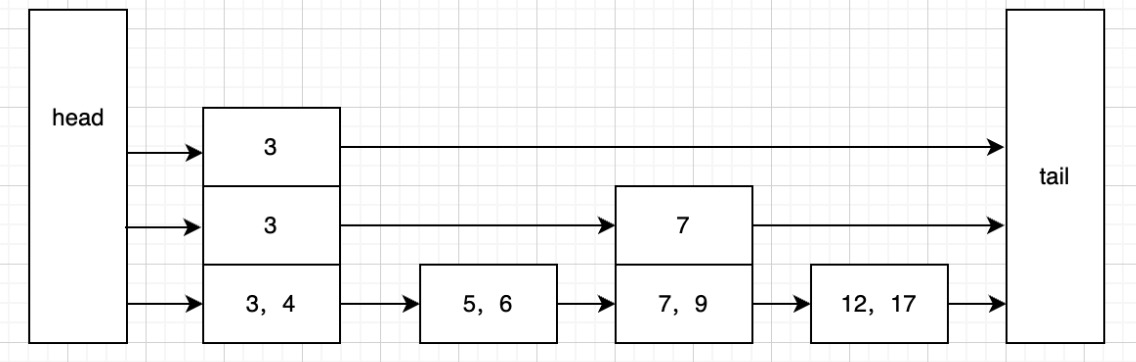
\includegraphics[width=0.9\columnwidth]{skiplist.png} % Assuming skiplist.png exists
\caption{A conceptual view of the Simple Cache-Sensitive Skip List (SCSSL) where data nodes (level 0) store arrays of elements (e.g., max array size = 2 as depicted). Index nodes point to the start of these arrays.}
\label{fig:conceptual_scssl}
\end{figure}

Our key contributions include:
\begin{enumerate}
    \item Introducing arrays within data-level nodes, which maintains the asymptotic complexity of skip list operations while significantly improving CPU cache hit rates due to the contiguous storage of multiple elements.
    \item Reducing the effective height of the skip list and pointer overhead, as each data-level node now stores multiple elements, leading to fewer nodes overall for a given dataset size.
    \item Presenting modified insertion, search, and deletion algorithms tailored for these array-based data nodes, offering a practical and simple approach for enhancing skip list performance, particularly in database indexing and similar applications.
\end{enumerate}

\section{Algorithms}
\label{sec:algorithms}
This section details the algorithms for search, insertion, and deletion in SCSSL. These operations are adapted from standard skip list algorithms to accommodate the array-based nodes at the data level.

In SCSSL, each node at the data level (level 0) stores its elements in a sorted array of a fixed maximum size. When a new node is created, its level is chosen randomly, similar to a standard skip list. A node promoted to level $k$ has $k+1$ forward pointers (indexed 0 to $k$). The maximum number of levels in the skip list is a predefined constant, `MAX_POSSIBLE_LEVEL`. The skip list employs a header node to initiate searches; its forward pointers are initially \Nil. For simplicity in comparisons, the header node can be conceptually considered to hold a key value of negative infinity or have a special marker.

Figure \ref{fig:insertion_example} illustrates an example of an insertion operation in SCSSL.

% TODO: This TikZ figure might be too wide for a two-column format.
% Consider using \resizebox{\columnwidth}{!}{...} or adjusting internal scaling.
\begin{figure}[htbp]
\centering
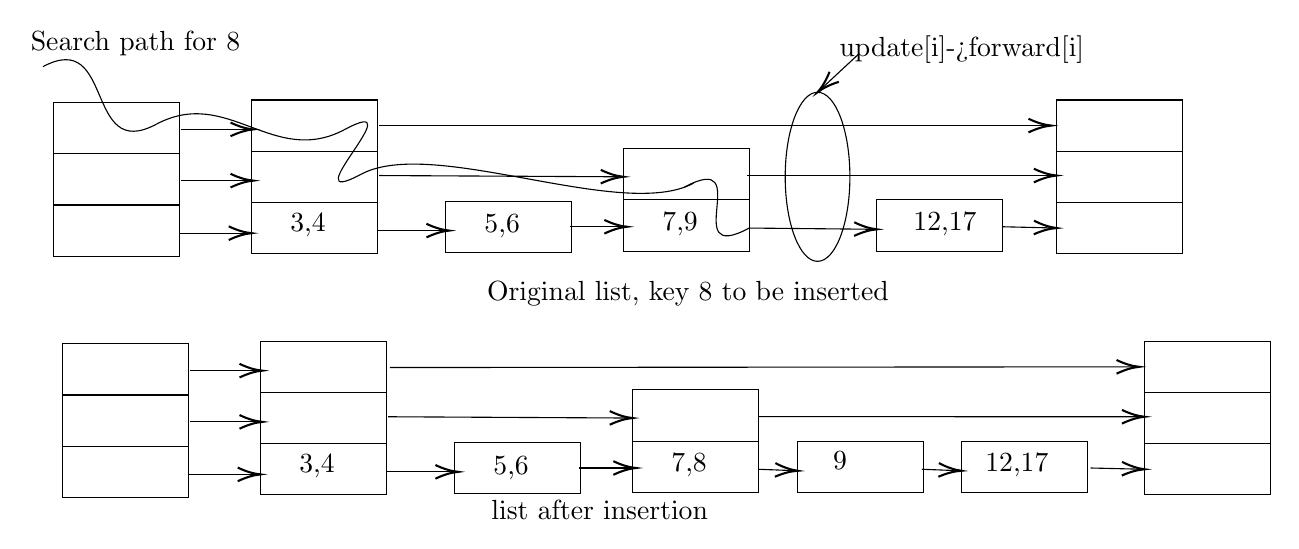
\begin{tikzpicture}[x=0.75pt,y=0.75pt,yscale=-1,xscale=1] 
% ... (TikZ code as before, ensure no non-breaking spaces are present) ...
%Shape: Rectangle [id:dp802121456728152] 
\draw (57.79,105.64) -- (118.41,105.64) -- (118.41,130.32) -- (57.79,130.32) -- cycle ;
%Shape: Rectangle [id:dp9825705095547612] 
\draw (332.28,103.17) -- (392.89,103.17) -- (392.89,127.86) -- (332.28,127.86) -- cycle ;
%Shape: Rectangle [id:dp248949237262718] 
\draw (246.56,103.79) -- (307.17,103.79) -- (307.17,128.47) -- (246.56,128.47) -- cycle ;
%Shape: Rectangle [id:dp1628354408576529] 
\draw (153.04,104.41) -- (213.65,104.41) -- (213.65,129.09) -- (153.04,129.09) -- cycle ;
%Shape: Rectangle [id:dp000018829587681290505] 
\draw (57.79,56.27) -- (118.41,56.27) -- (118.41,80.96) -- (57.79,80.96) -- cycle ;
%Shape: Rectangle [id:dp247562625981687] 
\draw (57.79,80.96) -- (118.41,80.96) -- (118.41,105.64) -- (57.79,105.64) -- cycle ;
%Shape: Rectangle [id:dp2644216550992282] 
\draw (540.96,104.41) -- (601.57,104.41) -- (601.57,129.09) -- (540.96,129.09) -- cycle ;
%Shape: Rectangle [id:dp8347359895416517] 
\draw (540.96,55.04) -- (601.57,55.04) -- (601.57,79.72) -- (540.96,79.72) -- cycle ;
%Shape: Rectangle [id:dp6823901202027933] 
\draw (540.96,79.72) -- (601.57,79.72) -- (601.57,104.41) -- (540.96,104.41) -- cycle ;
%Shape: Rectangle [id:dp379773497534003] 
\draw (153.04,79.72) -- (213.65,79.72) -- (213.65,104.41) -- (153.04,104.41) -- cycle ;
%Shape: Rectangle [id:dp8262463980956687] 
\draw (153.04,55.04) -- (213.65,55.04) -- (213.65,79.72) -- (153.04,79.72) -- cycle ;
%Shape: Rectangle [id:dp618442800182132] 
\draw (454.37,103.17) -- (514.98,103.17) -- (514.98,127.86) -- (454.37,127.86) -- cycle ;
%Straight Lines [id:da18234761053431092] 
\draw (118.41,119.22) -- (151.04,119.22) ;
\draw [shift={(153.04,119.22)}, rotate = 180] [color={rgb, 255:red, 0; green, 0; blue, 0 }][line width=0.75] (10.93,-3.29) .. controls (6.95,-1.4) and (3.31,-0.3) .. (0,0) .. controls (3.31,0.3) and (6.95,1.4) .. (10.93,3.29) ;
%Straight Lines [id:da17691354593928432] 
\draw (213.65,117.98) -- (246.29,117.98) ;
\draw [shift={(248.29,117.98)}, rotate = 180] [color={rgb, 255:red, 0; green, 0; blue, 0 }][line width=0.75] (10.93,-3.29) .. controls (6.95,-1.4) and (3.31,-0.3) .. (0,0) .. controls (3.31,0.3) and (6.95,1.4) .. (10.93,3.29) ;
%Straight Lines [id:da06545360607750506] 
\draw (306.3,116.13) -- (332.01,116.13) ;
\draw [shift={(334.01,116.13)}, rotate = 180] [color={rgb, 255:red, 0; green, 0; blue, 0 }][line width=0.75] (10.93,-3.29) .. controls (6.95,-1.4) and (3.31,-0.3) .. (0,0) .. controls (3.31,0.3) and (6.95,1.4) .. (10.93,3.29) ;
%Straight Lines [id:da8917793267177494] 
\draw (392.89,116.75) -- (452.37,117.34) ;
\draw [shift={(454.37,117.36)}, rotate = 180.58] [color={rgb, 255:red, 0; green, 0; blue, 0 }][line width=0.75] (10.93,-3.29) .. controls (6.95,-1.4) and (3.31,-0.3) .. (0,0) .. controls (3.31,0.3) and (6.95,1.4) .. (10.93,3.29) ;
%Straight Lines [id:da6270688079351094] 
\draw (514.98,116.13) -- (538.96,116.7) ;
\draw [shift={(540.96,116.75)}, rotate = 181.36] [color={rgb, 255:red, 0; green, 0; blue, 0 }][line width=0.75] (10.93,-3.29) .. controls (6.95,-1.4) and (3.31,-0.3) .. (0,0) .. controls (3.31,0.3) and (6.95,1.4) .. (10.93,3.29) ;
%Straight Lines [id:da16483082426708995] 
\draw (119.27,93.91) -- (151.91,93.91) ;
\draw [shift={(153.91,93.91)}, rotate = 180] [color={rgb, 255:red, 0; green, 0; blue, 0 }][line width=0.75] (10.93,-3.29) .. controls (6.95,-1.4) and (3.31,-0.3) .. (0,0) .. controls (3.31,0.3) and (6.95,1.4) .. (10.93,3.29) ;
%Shape: Rectangle [id:dp8280971824764716] 
\draw (332.28,78.49) -- (392.89,78.49) -- (392.89,103.17) -- (332.28,103.17) -- cycle ;
%Straight Lines [id:da6251582090553987] 
\draw (119.27,69.23) -- (151.91,69.23) ;
\draw [shift={(153.91,69.23)}, rotate = 180] [color={rgb, 255:red, 0; green, 0; blue, 0 }][line width=0.75] (10.93,-3.29) .. controls (6.95,-1.4) and (3.31,-0.3) .. (0,0) .. controls (3.31,0.3) and (6.95,1.4) .. (10.93,3.29) ;
%Straight Lines [id:da906622887317923] 
\draw (214.52,67.38) -- (536.36,67.38) ;
\draw [shift={(538.36,67.38)}, rotate = 180] [color={rgb, 255:red, 0; green, 0; blue, 0 }][line width=0.75] (10.93,-3.29) .. controls (6.95,-1.4) and (3.31,-0.3) .. (0,0) .. controls (3.31,0.3) and (6.95,1.4) .. (10.93,3.29) ;
%Straight Lines [id:da1247883464855224] 
\draw (214.52,91.45) -- (330.28,92.05) ;
\draw [shift={(332.28,92.06)}, rotate = 180.3] [color={rgb, 255:red, 0; green, 0; blue, 0 }][line width=0.75] (10.93,-3.29) .. controls (6.95,-1.4) and (3.31,-0.3) .. (0,0) .. controls (3.31,0.3) and (6.95,1.4) .. (10.93,3.29) ;
%Straight Lines [id:da5312111106538793] 
\draw (392.03,91.45) -- (538.96,91.45) ;
\draw [shift={(540.96,91.45)}, rotate = 180] [color={rgb, 255:red, 0; green, 0; blue, 0 }][line width=0.75] (10.93,-3.29) .. controls (6.95,-1.4) and (3.31,-0.3) .. (0,0) .. controls (3.31,0.3) and (6.95,1.4) .. (10.93,3.29) ;
%Curve Lines [id:da7690346774156931] 
\draw (107.15,66.76) .. controls (141.78,48.25) and (163.43,87.74) .. (198.07,69.23) ;
%Curve Lines [id:da09969258339888487] 
\draw (198.07,69.23) .. controls (232.7,50.72) and (171.22,109.34) .. (205.86,90.83) ;
%Curve Lines [id:da17301735066569246] 
\draw (205.86,90.83) .. controls (240.5,72.32) and (331.41,113.66) .. (366.05,95.15) ;
%Curve Lines [id:da04935924618461396] 
\draw (361.72,97) .. controls (396.36,78.49) and (358.26,135.26) .. (392.89,116.75) ;
%Curve Lines [id:da43861108104506963] 
\draw (52.6,38.99) .. controls (87.23,20.48) and (72.51,85.27) .. (107.15,66.76) ;
%Shape: Ellipse [id:dp551323556779669] 
\draw (410.21,92.06) .. controls (410.21,69.57) and (417.19,51.33) .. (425.8,51.33) .. controls (434.4,51.33) and (441.38,69.57) .. (441.38,92.06) .. controls (441.38,114.56) and (434.4,132.79) .. (425.8,132.79) .. controls (417.19,132.79) and (410.21,114.56) .. (410.21,92.06) -- cycle ;
%Straight Lines [id:da9115207752269137] 
\draw (445.71,32.82) -- (427.26,49.97) ;
\draw [shift={(425.8,51.33)}, rotate = 317.09] [color={rgb, 255:red, 0; green, 0; blue, 0 }][line width=0.75] (10.93,-3.29) .. controls (6.95,-1.4) and (3.31,-0.3) .. (0,0) .. controls (3.31,0.3) and (6.95,1.4) .. (10.93,3.29) ;
%Shape: Rectangle [id:dp44944938443713855] 
\draw (62.12,221.87) -- (122.73,221.87) -- (122.73,246.55) -- (62.12,246.55) -- cycle ;
%Shape: Rectangle [id:dp8751335667917544] 
\draw (336.61,219.4) -- (397.22,219.4) -- (397.22,244.08) -- (336.61,244.08) -- cycle ;
%Shape: Rectangle [id:dp2257346710215089] 
\draw (250.89,220.01) -- (311.5,220.01) -- (311.5,244.7) -- (250.89,244.7) -- cycle ;
%Shape: Rectangle [id:dp8771184949651254] 
\draw (157.37,220.63) -- (217.98,220.63) -- (217.98,245.32) -- (157.37,245.32) -- cycle ;
%Shape: Rectangle [id:dp5789469841235695] 
\draw (62.12,172.5) -- (122.73,172.5) -- (122.73,197.18) -- (62.12,197.18) -- cycle ;
%Shape: Rectangle [id:dp5624687649592586] 
\draw (62.12,197.18) -- (122.73,197.18) -- (122.73,221.87) -- (62.12,221.87) -- cycle ;
%Shape: Rectangle [id:dp13120546674792055] 
\draw (583.39,220.63) -- (644,220.63) -- (644,245.32) -- (583.39,245.32) -- cycle ;
%Shape: Rectangle [id:dp18910975661576046] 
\draw (583.39,171.26) -- (644,171.26) -- (644,195.95) -- (583.39,195.95) -- cycle ;
%Shape: Rectangle [id:dp968839873549274] 
\draw (583.39,195.95) -- (644,195.95) -- (644,220.63) -- (583.39,220.63) -- cycle ;
%Shape: Rectangle [id:dp5100738159249718] 
\draw (157.37,195.95) -- (217.98,195.95) -- (217.98,220.63) -- (157.37,220.63) -- cycle ;
%Shape: Rectangle [id:dp5130816669129519] 
\draw (157.37,171.26) -- (217.98,171.26) -- (217.98,195.95) -- (157.37,195.95) -- cycle ;
%Shape: Rectangle [id:dp10069788621732956] 
\draw (495.07,219.4) -- (555.68,219.4) -- (555.68,244.08) -- (495.07,244.08) -- cycle ;
%Straight Lines [id:da7506949131852723] 
\draw (122.73,235.44) -- (155.37,235.44) ;
\draw [shift={(157.37,235.44)}, rotate = 180] [color={rgb, 255:red, 0; green, 0; blue, 0 }][line width=0.75] (10.93,-3.29) .. controls (6.95,-1.4) and (3.31,-0.3) .. (0,0) .. controls (3.31,0.3) and (6.95,1.4) .. (10.93,3.29) ;
%Straight Lines [id:da5055411274108006] 
\draw (217.98,234.21) -- (250.62,234.21) ;
\draw [shift={(252.62,234.21)}, rotate = 180] [color={rgb, 255:red, 0; green, 0; blue, 0 }][line width=0.75] (10.93,-3.29) .. controls (6.95,-1.4) and (3.31,-0.3) .. (0,0) .. controls (3.31,0.3) and (6.95,1.4) .. (10.93,3.29) ;
%Straight Lines [id:da7559298876477776] 
\draw (310.63,232.36) -- (336.34,232.36) ;
\draw [shift={(338.34,232.36)}, rotate = 180] [color={rgb, 255:red, 0; green, 0; blue, 0 }][line width=0.75] (10.93,-3.29) .. controls (6.95,-1.4) and (3.31,-0.3) .. (0,0) .. controls (3.31,0.3) and (6.95,1.4) .. (10.93,3.29) ;
%Straight Lines [id:da08581070094109111] 
\draw (397.22,232.97) -- (414.27,233.62) ;
\draw [shift={(416.27,233.7)}, rotate = 182.18] [color={rgb, 255:red, 0; green, 0; blue, 0 }][line width=0.75] (10.93,-3.29) .. controls (6.95,-1.4) and (3.31,-0.3) .. (0,0) .. controls (3.31,0.3) and (6.95,1.4) .. (10.93,3.29) ;
%Straight Lines [id:da5858905620692174] 
\draw (557.41,232.36) -- (581.39,232.93) ;
\draw [shift={(583.39,232.97)}, rotate = 181.36] [color={rgb, 255:red, 0; green, 0; blue, 0 }][line width=0.75] (10.93,-3.29) .. controls (6.95,-1.4) and (3.31,-0.3) .. (0,0) .. controls (3.31,0.3) and (6.95,1.4) .. (10.93,3.29) ;
%Straight Lines [id:da32674036346427937] 
\draw (123.6,210.14) -- (156.24,210.14) ;
\draw [shift={(158.24,210.14)}, rotate = 180] [color={rgb, 255:red, 0; green, 0; blue, 0 }][line width=0.75] (10.93,-3.29) .. controls (6.95,-1.4) and (3.31,-0.3) .. (0,0) .. controls (3.31,0.3) and (6.95,1.4) .. (10.93,3.29) ;
%Shape: Rectangle [id:dp026479095509071682] 
\draw (336.61,194.71) -- (397.22,194.71) -- (397.22,219.4) -- (336.61,219.4) -- cycle ;
%Straight Lines [id:da5236391813651351] 
\draw (123.6,185.46) -- (156.24,185.46) ;
\draw [shift={(158.24,185.46)}, rotate = 180] [color={rgb, 255:red, 0; green, 0; blue, 0 }][line width=0.75] (10.93,-3.29) .. controls (6.95,-1.4) and (3.31,-0.3) .. (0,0) .. controls (3.31,0.3) and (6.95,1.4) .. (10.93,3.29) ;
%Straight Lines [id:da951241427709963] 
\draw (219.71,183.96) -- (578.79,183.61) ;
\draw [shift={(580.79,183.61)}, rotate = 179.94] [color={rgb, 255:red, 0; green, 0; blue, 0 }][line width=0.75] (10.93,-3.29) .. controls (6.95,-1.4) and (3.31,-0.3) .. (0,0) .. controls (3.31,0.3) and (6.95,1.4) .. (10.93,3.29) ;
%Straight Lines [id:da5677734486818795] 
\draw (218.85,207.67) -- (334.61,208.28) ;
\draw [shift={(336.61,208.29)}, rotate = 180.3] [color={rgb, 255:red, 0; green, 0; blue, 0 }][line width=0.75] (10.93,-3.29) .. controls (6.95,-1.4) and (3.31,-0.3) .. (0,0) .. controls (3.31,0.3) and (6.95,1.4) .. (10.93,3.29) ;
%Straight Lines [id:da03778045413284792] 
\draw (397.22,207.61) -- (581.39,207.67) ;
\draw [shift={(583.39,207.67)}, rotate = 180.02] [color={rgb, 255:red, 0; green, 0; blue, 0 }][line width=0.75] (10.93,-3.29) .. controls (6.95,-1.4) and (3.31,-0.3) .. (0,0) .. controls (3.31,0.3) and (6.95,1.4) .. (10.93,3.29) ;
%Shape: Rectangle [id:dp9874088035206192] 
\draw (416.27,219.4) -- (476.88,219.4) -- (476.88,244.08) -- (416.27,244.08) -- cycle ;
%Straight Lines [id:da719219755060643] 
\draw (476.02,232.97) -- (493.07,233.62) ;
\draw [shift={(495.07,233.7)}, rotate = 182.18] [color={rgb, 255:red, 0; green, 0; blue, 0 }][line width=0.75] (10.93,-3.29) .. controls (6.95,-1.4) and (3.31,-0.3) .. (0,0) .. controls (3.31,0.3) and (6.95,1.4) .. (10.93,3.29) ;

% Text Node
\draw (170.55,108.56) node [anchor=north west][inner sep=0.75pt] [align=left] {3,4};
% Text Node
\draw (264.06,109.17) node [anchor=north west][inner sep=0.75pt] [align=left] {5,6};
% Text Node
\draw (349.79,107.94) node [anchor=north west][inner sep=0.75pt] [align=left] {7,9};
% Text Node
\draw (470.74,107.94) node [anchor=north west][inner sep=0.75pt] [align=left] {12,17};
% Text Node
\draw (45.5,20.51) node [anchor=north west][inner sep=0.75pt] [align=left] {Search path for 8};
% Text Node
\draw (435.12,22.78) node [anchor=north west][inner sep=0.75pt] [align=left] {update[i]->forward[i]};
% Text Node
\draw (265.32,141.26) node [anchor=north west][inner sep=0.75pt] [align=left] {Original list, key 8 to be inserted};
% Text Node
\draw (174.88,224.78) node [anchor=north west][inner sep=0.75pt] [align=left] {3,4};
% Text Node
\draw (268.39,225.4) node [anchor=north west][inner sep=0.75pt] [align=left] {5,6};
% Text Node
\draw (354.12,224.17) node [anchor=north west][inner sep=0.75pt] [align=left] {7,8}; % Node modified
% Text Node
\draw (505.37,224.17) node [anchor=north west][inner sep=0.75pt] [align=left] {12,17};
\draw (431.99,223.16) node [anchor=north west][inner sep=0.75pt] [align=left] {9}; % New node contains 9
% Text Node -- Corrected typo from original paper
\draw (267.41,246.44) node [anchor=north west][inner sep=0.75pt] [align=left] {list after insertion};
\end{tikzpicture}
\caption{Insertion of key 8 into an SCSSL (max array size = 2). Key 8 displaces 9 from node (7,9). Key 9 is then inserted into a new node.}
\label{fig:insertion_example}
\end{figure}

\subsection{Initialization}
The initialization process is elementary. A header node is created with an array of `MAX_POSSIBLE_LEVEL + 1` forward pointers, all initialized to \Nil. To simplify comparisons, the header node's key array (if it were to have one in the same structure) can be considered to contain a single sentinel value of negative infinity, or it can be handled as a special case. In our algorithms, `header.FirstKey()` would effectively be $-\infty$.

\subsection{Search}
The search algorithm (Algorithm \ref{alg:search}) navigates the skip list from the highest level down to level 0. At each level `i`, it traverses forward as long as the first key of the array in the next node (`current.forward[i].FirstKey()`) is less than or equal to the search key `k`. Once this traversal is complete, the `current` node is the one whose own array might contain `k` (specifically, `current.FirstKey() <= k`, and either `current.forward[0]` is \Nil or `current.forward[0].FirstKey() > k`). The final step involves searching for `k` within `current`'s array.

\begin{algorithm}[htbp] % Changed [H] to [htbp]
    \caption{Search for Key $k$ in SCSSL}
    \label{alg:search}
    \KwIn{Search key $k$, current global maximum level `currentGlobalMaxLevel`, header node `header`}
    \KwOut{Node containing key $k$ and its index in array, or (\Nil, -1) if not found}
    \SetKwFunction{FSearch}{Search}
    \SetKwProg{Fn}{Function}{:}{}
    \Fn{\FSearch{$k$, currentGlobalMaxLevel, header}}{
        $current \gets header$\;
        \For{$i \gets \text{currentGlobalMaxLevel}$ \KwDownTo $0$}{
            \While{$current.forward[i] \neq \Nil \land current.forward[i].FirstKey() \leq k$}{
                $current \gets current.forward[i]$\;
            }
        }
        \Return $current.\text{search\_in\_array}(k)$\; \tcp{Returns (node, index) or (\Nil, -1)}
    }
\end{algorithm}

\subsection{Insertion}
The insertion algorithm (Algorithm \ref{alg:insert}) first searches for the appropriate position for the new key `k`, maintaining an `update` array to store pointers to the predecessor nodes at each level. The core logic then addresses several cases based on whether the target data node (`target_node`, which is `update[0]`) can accommodate `k`:
% ... (itemize description as before) ...
\begin{itemize}
    \item \textbf{Current node is header:} If `target_node` is the header, a new node is usually created, or `k` is inserted into `header.forward[0]` if conditions permit.
    \item \textbf{Target node full, `k` fits within existing range (CASE 1 from paper):} If `target_node`'s array is full but `k` is smaller than its largest element (`target_node.array_last_element()`) and `k` is not smaller than its first element, the largest element is popped (`replaced_key`), `k` is inserted into `target_node`'s array, and the `replaced_key` becomes the new key to be inserted.
    \item \textbf{Target node not full (CASE 2 from paper):} If `target_node`'s array is not full and `k` belongs there (i.e., `k >= target_node.FirstKey()`), `k` is inserted directly into `target_node`'s array. The operation then completes.
    \item \textbf{Key `k` belongs after `target_node` (CASE 3 from paper):} If `k` is greater than all elements in `target_node`'s array (`k > target_node.array_last_element()`), insertion is attempted in `target_node.forward[0]`. If `target_node.forward[0]` is suitable (exists and not full and `k` is not smaller than its first key), `k` is inserted there.
    \item \textbf{New node creation (Other CASES):} If none of the above conditions lead to an in-place insertion, a new node is created for `k`. Its level is randomly determined. If this new level exceeds the list's `currentGlobalMaxLevel`, the `update` array and `currentGlobalMaxLevel` are adjusted. Pointers are then updated to link the new node.
\end{itemize}


\begin{algorithm}[htbp] % Changed [H] to [htbp]
    \caption{Insert Key $k$ into SCSSL}
    \label{alg:insert}
    \KwIn{Key $k$, current global maximum level `currentGlobalMaxLevel`, header node `header`, constant `MAX_POSSIBLE_LEVEL`}
    \KwOut{Potentially updated `currentGlobalMaxLevel`}
    \SetKwFunction{FInsert}{Insert}
    \SetKwProg{Fn}{Function}{:}{}
    \Fn{\FInsert{$k$, currentGlobalMaxLevel, header, MAX\_POSSIBLE\_LEVEL}}{
        $update[\text{MAX\_POSSIBLE\_LEVEL + 1}]$ \tcp*{Array to store predecessors}
        $current \gets header$\;
        
        \For{$i \gets \text{currentGlobalMaxLevel}$ \KwDownTo $0$}{
            \While{$current.forward[i] \neq \Nil \land current.forward[i].FirstKey() \leq k$}{
                $current \gets current.forward[i]$\;
            }
            $update[i] \gets current$\;
        }
        
        $target\_node \gets update[0]$\;
        
        \If{$target\_node \neq header \land target\_node.is\_full() \land k < target\_node.array\_last\_element() \land k >= target\_node.FirstKey()$}{
            \tcp{CASE 1}
            $replaced\_key \gets target\_node.array.pop\_last()$\;
            $target\_node.insert\_into\_array(k)$\;
            $k \gets replaced\_key$\;
        }
        
        \If{$target\_node \neq header \land \neg target\_node.is\_full() \land k >= target\_node.FirstKey()$}{
            \tcp{CASE 2}
            $target\_node.insert\_into\_array(k)$\;
            \KwRet currentGlobalMaxLevel\; \tcp{Insertion complete}
        }

        $current \gets target\_node.forward[0]$\; 
        \If{$current \neq \Nil \land \neg current.is\_full() \land k >= current.FirstKey() $}{
            \tcp{CASE 3}
            $current.insert\_into\_array(k)$\;
            \KwRet currentGlobalMaxLevel\; \tcp{Insertion complete}
        }
        \Else{ \tcp{OTHER CASES: Create a new node for k}
            $new\_node\_level \gets \text{random\_level}()$\;
            
            \If{$new\_node\_level > \text{currentGlobalMaxLevel}$}{
                \For{$i \gets \text{currentGlobalMaxLevel} + 1$ \KwTo $new\_node\_level$}{
                    $update[i] \gets header$\;
                }
                $\text{currentGlobalMaxLevel} \gets new\_node\_level$\;
            }
            
            $new\_node \gets \text{Node}([k], \text{new\_node\_level})$\;
            
            \For{$i \gets 0 $ \KwTo $new\_node\_level$}{
                $new\_node.forward[i] \gets update[i].forward[i]$\;
                $update[i].forward[i] \gets new\_node$\;
            }
        }
        \KwRet currentGlobalMaxLevel\;
    }
\end{algorithm}

\subsection{Deletion}
The deletion algorithm (Algorithm \ref{alg:delete}) also starts by finding the key `k`. The traversal logic advances `current` as long as the *entire array* in `current.forward[i]` contains keys strictly smaller than `k` (i.e., `current.forward[i].array_last_element() < k`). This ensures that `update[0].forward[0]` becomes the first node whose array could potentially contain `k`.
% ... (itemize description as before) ...
If `k` is found and deleted from this node's array:
\begin{itemize}
    \item If the array becomes empty, the node itself is removed from the skip list by adjusting the forward pointers of its predecessors.
    \item If removing a node causes some highest levels to become empty, `currentGlobalMaxLevel` is decremented.
\end{itemize}

\begin{algorithm}[htbp] % Changed [H] to [htbp]
    \caption{Delete Key $k$ from SCSSL}
    \label{alg:delete}
    \KwIn{Key $k$, current global maximum level `currentGlobalMaxLevel`, header node `header`, constant `MAX_POSSIBLE_LEVEL`}
    \KwOut{(Boolean indicating success, potentially updated `currentGlobalMaxLevel`)}
    \SetKwFunction{FDelete}{Delete}
    \SetKwProg{Fn}{Function}{:}{}
    \Fn{\FDelete{$k$, currentGlobalMaxLevel, header, MAX\_POSSIBLE\_LEVEL}}{
        $update[\text{MAX\_POSSIBLE\_LEVEL + 1}]$\;
        $current \gets header$\;
        
        \For{$i \gets \text{currentGlobalMaxLevel}$ \KwDownTo $0$}{
            \While{$current.forward[i] \neq \Nil \land current.forward[i].array\_last\_element() < k$}{
                $current \gets current.forward[i]$\;
            }
            $update[i] \gets current$\;
        }
        
        $node\_to\_check \gets current.forward[0]$\;
        \If{$node\_to\_check = \Nil$}{
            \KwRet{ (False, currentGlobalMaxLevel) }\;
        }
        
        \If{$k < node\_to\_check.FirstKey()$}{
             \KwRet{ (False, currentGlobalMaxLevel) }\;
        }

        $deleted\_from\_arr \gets node\_to\_check.delete\_from\_array(k)$\;
        \If{$\neg deleted\_from\_arr$}{
            \KwRet{ (False, currentGlobalMaxLevel) }\;
        }
        
        \If{$node\_to\_check.is\_array\_empty()$}{
            \For{$i \gets 0$ \KwTo $node\_to\_check.level$}{
                \If{$update[i].forward[i] \neq node\_to\_check$}{
                    \Break\;
                }
                $update[i].forward[i] \gets node\_to\_check.forward[i]$\;
            }
            % Deallocate node_to_check (memory management implied)
            \While{$\text{currentGlobalMaxLevel} > 0 \land header.forward[\text{currentGlobalMaxLevel}] = \Nil$}{
                $\text{currentGlobalMaxLevel} \gets \text{currentGlobalMaxLevel} - 1$\;
            }
        }
        \KwRet{ (True, currentGlobalMaxLevel) }\;
    }
\end{algorithm}

\section{Experimental Evaluation}
\label{sec:evaluation}

\subsection{Experimental Environment}
The experiments were conducted in the following environments:
\begin{itemize}
    \item \textbf{Hardware 1 (MacBook):} Apple M2 CPU, 16 GB RAM.
    \item \textbf{Hardware 2 (Server):} Intel(R) Core(TM) i7-6700 CPU @ 3.40GHz, 24 GB DDR4 2133 MHz RAM. This server was used not only for performance testing but also specifically for analyzing CPU cache miss rates using appropriate profiling tools (e.g., `perf`).
    \item \textbf{Compiler:} The algorithms were implemented in C++. The test programs were compiled using g++ (version specific to environment, e.g., 9.0 or higher) with the `-O3` optimization flag.
    \item \textbf{Benchmark Configuration:}
        Insertion operations in a skip list are prone to CPU cache misses due to dynamic memory allocations and pointer chasing. Therefore, our benchmarks primarily focus on insertion performance using randomly generated integer keys. The number of elements ranged from 100 to 300,000.
        Search performance was also evaluated. However, we do not present detailed search results as the performance difference between SCSSL and the standard skip list was found to be negligible for typical search operations. This is likely because the dominant factor in search is the traversal of levels, which has a similar path length, and the final array scan in SCSSL is very fast for small arrays.
        Both the standard skip list and SCSSL were configured with a maximum level (`MAX_POSSIBLE_LEVEL`) of 16. For SCSSL, the maximum array size within a data node was set to a value empirically found to be effective (e.g., 64 or 128, chosen to fit well within L1 cache lines).
\end{itemize}

\subsection{Results and Discussion}

\begin{figure}[htbp]
\centering
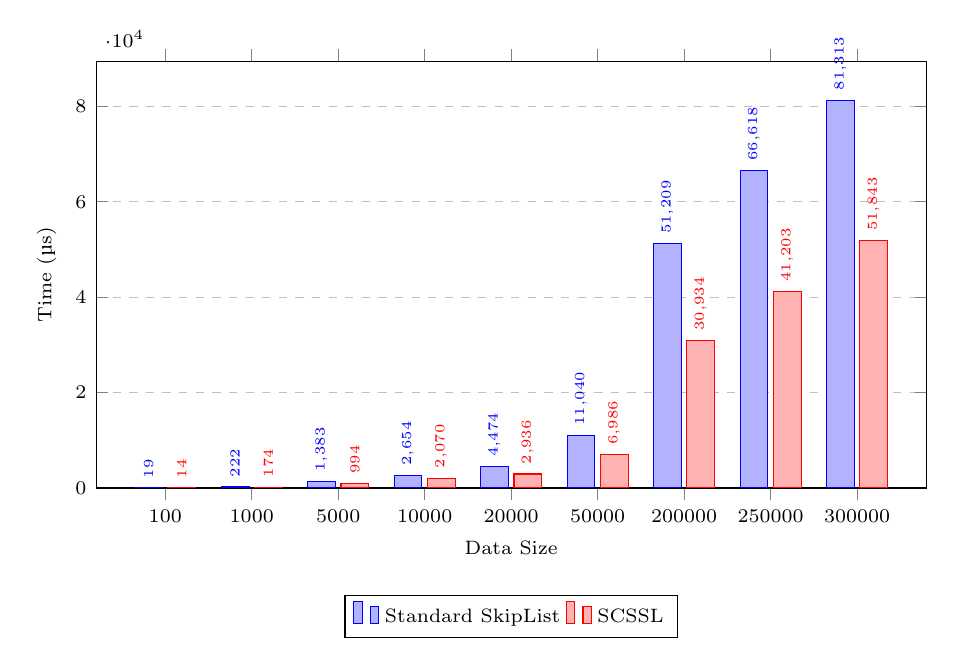
\begin{tikzpicture}
\begin{axis}[
    ybar,
    bar width=10pt,
    width=\columnwidth, % Adjusted for two-column
    height=7cm, % Slightly reduced height for better fit
    enlarge x limits=0.1,
    xlabel={Data Size},
    ylabel={Time (\textmu s)},
    symbolic x coords={100,1000,5000,10000,20000,50000,200000,250000,300000},
    xtick=data,
    legend style={at={(0.5,-0.25)},anchor=north,legend columns=2, font=\scriptsize}, % Adjusted legend
    nodes near coords,
    every node near coord/.append style={font=\tiny, rotate=90, anchor=west},
    ymin=0,
    ymajorgrids=true,
    grid style=dashed,
    label style={font=\scriptsize}, % Smaller axis labels
    tick label style={font=\scriptsize} % Smaller tick labels
]
\addplot+[style={blue,fill=blue!30}] coordinates {
    (100,19) (1000,222) (5000,1383) (10000,2654) (20000,4474) (50000,11040) (200000,51209) (250000,66618) (300000,81313)
};
\addplot+[style={red,fill=red!30}] coordinates {
    (100,14) (1000,174) (5000,994) (10000,2070) (20000,2936) (50000,6986) (200000,30934) (250000,41203) (300000,51843)
};
\legend{Standard SkipList, SCSSL}
\end{axis}
\end{tikzpicture}
\caption{Insertion Time Comparison: Standard Skip List vs. SCSSL on macOS (Apple M2). Lower is better.}
\label{fig:perf_macos}
\end{figure}

\begin{figure}[htbp]
\centering
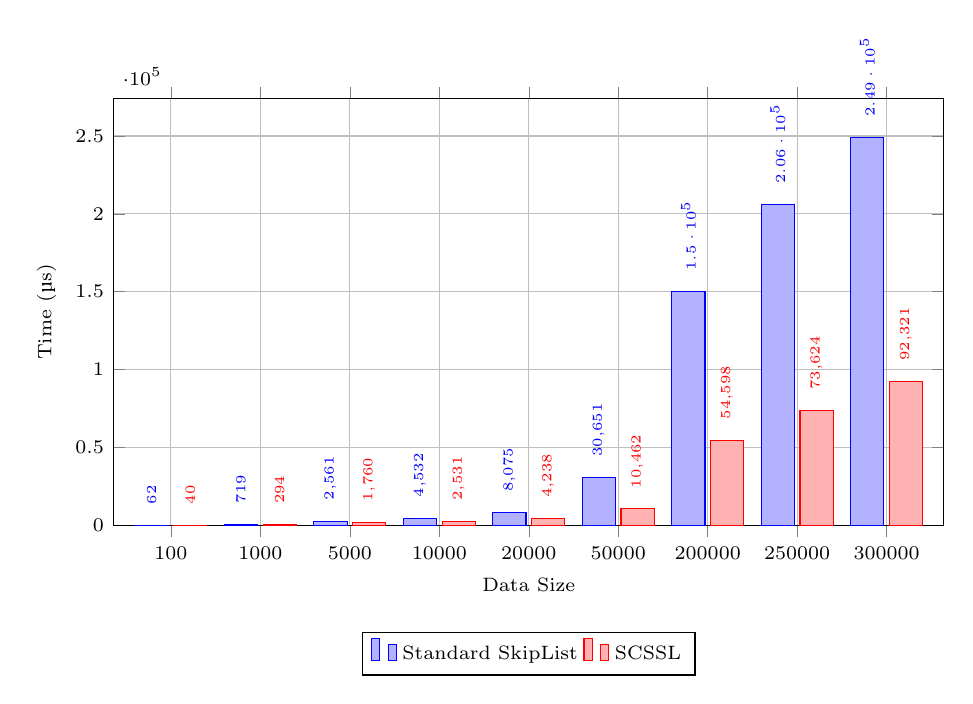
\begin{tikzpicture}
\begin{axis}[
    width=\columnwidth, % Adjusted for two-column
    height=7cm, % Slightly reduced height
    ybar,
    bar width=12pt,
    symbolic x coords={100,1000,5000,10000,20000,50000,200000,250000,300000},
    xtick=data,
    xlabel={Data Size},
    ylabel={Time (\textmu s)},
    legend style={at={(0.5,-0.25)},anchor=north,legend columns=-1, font=\scriptsize}, % Adjusted legend
    enlarge x limits=0.08,
    ymin=0,
    grid=major,
    nodes near coords,
    nodes near coords style={font=\tiny, anchor=west, rotate=90, xshift=4pt}, % Adjusted nodes near coords
    label style={font=\scriptsize},
    tick label style={font=\scriptsize}
]
\addplot coordinates {(100,62) (1000,719) (5000,2561) (10000,4532) (20000,8075) (50000,30651) (200000,150126) (250000,206036) (300000,249135)};
\addplot coordinates {(100,40) (1000,294) (5000,1760) (10000,2531) (20000,4238) (50000,10462) (200000,54598) (250000,73624) (300000,92321)};
\legend{Standard SkipList, SCSSL}
\end{axis}
\end{tikzpicture}
\caption{Insertion Time Comparison: Standard Skip List vs. SCSSL on Server (Intel i7-6700). Lower is better.}
\label{fig:perf_server}
\end{figure}

On the MacBook (Apple M2 processor, Figure \ref{fig:perf_macos}), SCSSL demonstrates a speedup of 1.28x-1.39x for small datasets (<1,000 elements) during insertion. For medium-scale datasets (>20,000 elements), the speedup increases to a range of 1.55x-1.65x. This trend indicates that the cache-friendly benefits of SCSSL become more pronounced as the dataset size grows, leading to more memory accesses.

On the server system (Intel i7-6700, Figure \ref{fig:perf_server}), SCSSL achieves even more significant speedups for insertions, reaching up to nearly 3x compared to the standard skip list for larger datasets (e.g., 300,000 elements). This enhanced improvement on the server platform might be attributed to differences in cache architecture, memory subsystem performance, or the relative cost of cache misses compared to the M2 architecture.

\begin{table}[htbp]
\centering
\caption{Cache Performance Comparison (Insertions, 300,000 elements) on Server (Intel i7-6700)}
\label{tab:cache_performance}
\begin{tabular}{@{}lrrr@{}}
\toprule
Test Case & Cache References & Cache Misses & Cache Miss Rate \\
\midrule
SCSSL & 51,567,218 & 459,636 & 0.89\% \\
Standard Skip List & 142,249,678 & 47,251,323 & 33.22\% \\
\bottomrule
\end{tabular}
\end{table}

Table \ref{tab:cache_performance} presents the cache performance data for inserting 300,000 random elements on the server. The standard skip list exhibits a high L1 data cache miss rate of 33.22\%. In contrast, SCSSL drastically reduces this rate to a mere 0.89\%. This substantial reduction in cache misses directly corroborates our hypothesis that embedding arrays within data nodes effectively improves data locality and cache utilization, which translates into the observed speedups. The significantly lower number of cache references for SCSSL also suggests more efficient data access patterns.

\section{Conclusion}
\label{sec:conclusion}

We have presented SCSSL, a novel cache-sensitive skip list variant that introduces a simple yet highly effective modification: replacing single elements in data-level nodes with small, sorted arrays. This architectural change allows SCSSL to enhance CPU cache performance by improving data locality, while crucially maintaining the algorithmic simplicity that is a hallmark of skip lists.

Experimental results demonstrate significant performance improvements for insertion operations, particularly on systems where cache performance is a critical factor. The observed speedups of 1.2x-3x, coupled with a dramatic reduction in cache miss rates (e.g., from 33.22\% to 0.89\% in our server tests), validate the efficacy of this approach. SCSSL offers a practical and easily implementable method to boost skip list performance in modern computing environments without resorting to complex algorithmic changes or specialized hardware features. Its simplicity makes it an attractive option for a wide range of applications, from embedded systems to large-scale in-memory data stores.

Future work could explore optimal array sizes for different hardware platforms and key/value types, as well as investigate the application of SCSSL principles in concurrent skip list implementations.

%%
%% The acknowledgments section is defined using the "acks" environment
%% (and NOT an unnumbered section). This ensures the proper
%% identification of the section in the article metadata, and the
%% consistent spelling of the heading.
% \begin{acks}
% To Robert, for the bagels and explaining CMYK and color spaces.
% \end{acks}

%%
%% The next two lines define the bibliography style to be used, and
%% the bibliography file.
\bibliographystyle{ACM-Reference-Format}
\bibliography{references} % Ensure you have references.bib file

%%
%% If your work has an appendix, this is the place to put it.
% \appendix
% \section{Research Methods}
% ...

\end{document}

% ======================================================================
% ====== IMPORTANT: Put the following content into a file ==========
% ====== named "references.bib" in the same directory as your .tex file ====
% ======================================================================
/*

@article{Pugh1990,
  author    = {Pugh, William},
  title     = {Skip Lists: {A} Probabilistic Alternative to Balanced Trees},
  journal   = {Communications of the ACM},
  volume    = {33},
  number    = {6},
  pages     = {668--676},
  year      = {1990},
  month     = jun,
  publisher = {ACM}
}

@misc{LevelDB,
  author    = {Google},
  title     = {{LevelDB}},
  howpublished = {\url{https://github.com/google/leveldb}},
  year      = {2011}, % Approx. year of public release for sorting
  note      = {Accessed on July 20, 2023}
}

@misc{Redis,
  author    = {{Redis Labs an Redis Community}}, % More accurate
  title     = {{Redis}},
  howpublished = {\url{https://redis.io}},
  year      = {2009}, % Initial release
  note      = {Accessed on January 09, 2024}
}

@misc{RocksDB,
  author    = {Meta Platforms, Inc. and community}, % More accurate
  title     = {{RocksDB}},
  howpublished = {\url{http://rocksdb.org/}},
  year      = {2012}, % Fork from LevelDB
  note      = {Accessed on July 20, 2023}
}

@misc{HBase,
  author = {{Apache Software Foundation}},
  title  = {Welcome to {Apache HBase}\textsuperscript{\texttrademark}},
  howpublished = {\url{https://hbase.apache.org/}},
  year   = {2008}, % Initial release, approximately
  note   = {Accessed on July 20, 2023}
}

@inproceedings{CSSL20XX, % Placeholder - User needs to find the actual publication
  author    = {Author, A. and Coauthor, B.}, % TODO: Replace with actual authors
  title     = {Cache-Sensitive Skip List: Efficient Range Queries on Modern CPUs},
  booktitle = {Proceedings of Some Conference or Journal Name}, % TODO: Replace with actual venue
  year      = {20XX}, % TODO: Replace with actual year
  note      = {Original reference source: informatik.hu-berlin.de. Actual publication details needed.}
}

@article{ESL20XX, % Corresponds to the MDPI link
  author    = {Liu, Yang and Zhang, Jian and Wang, Chao and Yu, Ge},
  title     = {{ESL}: {A} High-Performance Skiplist with Express Lane},
  journal   = {Applied Sciences},
  volume    = {13},
  number    = {17},
  pages     = {9925},
  year      = {2023},
  publisher = {MDPI AG},
  doi       = {10.3390/app13179925},
  URL       = {https://www.mdpi.com/2076-3417/13/17/9925}
}

*/
% ======================================================================
% ======================================================================